\section*{Supplementary Information}\label{supplementary-information}
\addcontentsline{toc}{section}{Supplementary Information}

\setcounter{table}{0} \renewcommand{\thetable}{S\arabic{table}}
\setcounter{figure}{0} \renewcommand{\thefigure}{S\arabic{figure}}

\begin{longtable}[]{@{}lllrlr@{}}
\caption{\label{tab:isolate-table} Description of \emph{Sclerotinia
sclerotiorum} isolates used in this study. N = Number of Isolates. Key
abbreviations: wmn = white mold screening nursery, producer = producer
field, unk = unknown cultivar.}\tabularnewline
\toprule
\begin{minipage}[b]{0.11\columnwidth}\raggedright\strut
Country\strut
\end{minipage} & \begin{minipage}[b]{0.08\columnwidth}\raggedright\strut
State\strut
\end{minipage} & \begin{minipage}[b]{0.12\columnwidth}\raggedright\strut
Field Code\strut
\end{minipage} & \begin{minipage}[b]{0.19\columnwidth}\raggedleft\strut
Year\strut
\end{minipage} & \begin{minipage}[b]{0.29\columnwidth}\raggedright\strut
Host\strut
\end{minipage} & \begin{minipage}[b]{0.04\columnwidth}\raggedleft\strut
N\strut
\end{minipage}\tabularnewline
\midrule
\endfirsthead
\toprule
\begin{minipage}[b]{0.11\columnwidth}\raggedright\strut
Country\strut
\end{minipage} & \begin{minipage}[b]{0.08\columnwidth}\raggedright\strut
State\strut
\end{minipage} & \begin{minipage}[b]{0.12\columnwidth}\raggedright\strut
Field Code\strut
\end{minipage} & \begin{minipage}[b]{0.19\columnwidth}\raggedleft\strut
Year\strut
\end{minipage} & \begin{minipage}[b]{0.29\columnwidth}\raggedright\strut
Host\strut
\end{minipage} & \begin{minipage}[b]{0.04\columnwidth}\raggedleft\strut
N\strut
\end{minipage}\tabularnewline
\midrule
\endhead
\begin{minipage}[t]{0.11\columnwidth}\raggedright\strut
USA\strut
\end{minipage} & \begin{minipage}[t]{0.08\columnwidth}\raggedright\strut
CA\strut
\end{minipage} & \begin{minipage}[t]{0.12\columnwidth}\raggedright\strut
wmn\strut
\end{minipage} & \begin{minipage}[t]{0.19\columnwidth}\raggedleft\strut
2004, 2005\strut
\end{minipage} & \begin{minipage}[t]{0.29\columnwidth}\raggedright\strut
Beryl, Bunsi, G122\strut
\end{minipage} & \begin{minipage}[t]{0.04\columnwidth}\raggedleft\strut
18\strut
\end{minipage}\tabularnewline
\begin{minipage}[t]{0.11\columnwidth}\raggedright\strut
USA\strut
\end{minipage} & \begin{minipage}[t]{0.08\columnwidth}\raggedright\strut
CO\strut
\end{minipage} & \begin{minipage}[t]{0.12\columnwidth}\raggedright\strut
producer\strut
\end{minipage} & \begin{minipage}[t]{0.19\columnwidth}\raggedleft\strut
2007, 2010\strut
\end{minipage} & \begin{minipage}[t]{0.29\columnwidth}\raggedright\strut
Pinto, Yellow\strut
\end{minipage} & \begin{minipage}[t]{0.04\columnwidth}\raggedleft\strut
41\strut
\end{minipage}\tabularnewline
\begin{minipage}[t]{0.11\columnwidth}\raggedright\strut
\strut
\end{minipage} & \begin{minipage}[t]{0.08\columnwidth}\raggedright\strut
\strut
\end{minipage} & \begin{minipage}[t]{0.12\columnwidth}\raggedright\strut
wmn\strut
\end{minipage} & \begin{minipage}[t]{0.19\columnwidth}\raggedleft\strut
2003\strut
\end{minipage} & \begin{minipage}[t]{0.29\columnwidth}\raggedright\strut
GH\strut
\end{minipage} & \begin{minipage}[t]{0.04\columnwidth}\raggedleft\strut
1\strut
\end{minipage}\tabularnewline
\begin{minipage}[t]{0.11\columnwidth}\raggedright\strut
USA\strut
\end{minipage} & \begin{minipage}[t]{0.08\columnwidth}\raggedright\strut
ID\strut
\end{minipage} & \begin{minipage}[t]{0.12\columnwidth}\raggedright\strut
producer\strut
\end{minipage} & \begin{minipage}[t]{0.19\columnwidth}\raggedleft\strut
2003\strut
\end{minipage} & \begin{minipage}[t]{0.29\columnwidth}\raggedright\strut
GH\strut
\end{minipage} & \begin{minipage}[t]{0.04\columnwidth}\raggedleft\strut
1\strut
\end{minipage}\tabularnewline
\begin{minipage}[t]{0.11\columnwidth}\raggedright\strut
USA\strut
\end{minipage} & \begin{minipage}[t]{0.08\columnwidth}\raggedright\strut
MI\strut
\end{minipage} & \begin{minipage}[t]{0.12\columnwidth}\raggedright\strut
wmn\strut
\end{minipage} & \begin{minipage}[t]{0.19\columnwidth}\raggedleft\strut
2003, 2004, 2005, 2008, 2009\strut
\end{minipage} & \begin{minipage}[t]{0.29\columnwidth}\raggedright\strut
11A, 37, 38, B07104, Beryl, Bunsi, Cornell, G122, Orion, PO7863,
WM31\strut
\end{minipage} & \begin{minipage}[t]{0.04\columnwidth}\raggedleft\strut
43\strut
\end{minipage}\tabularnewline
\begin{minipage}[t]{0.11\columnwidth}\raggedright\strut
\strut
\end{minipage} & \begin{minipage}[t]{0.08\columnwidth}\raggedright\strut
\strut
\end{minipage} & \begin{minipage}[t]{0.12\columnwidth}\raggedright\strut
producer\strut
\end{minipage} & \begin{minipage}[t]{0.19\columnwidth}\raggedleft\strut
2003, 2008, 2009\strut
\end{minipage} & \begin{minipage}[t]{0.29\columnwidth}\raggedright\strut
BL, Black, Fuji, GH, Merlot, SR06233, unk, Vista, Zorro\strut
\end{minipage} & \begin{minipage}[t]{0.04\columnwidth}\raggedleft\strut
19\strut
\end{minipage}\tabularnewline
\begin{minipage}[t]{0.11\columnwidth}\raggedright\strut
USA\strut
\end{minipage} & \begin{minipage}[t]{0.08\columnwidth}\raggedright\strut
MN\strut
\end{minipage} & \begin{minipage}[t]{0.12\columnwidth}\raggedright\strut
wmn\strut
\end{minipage} & \begin{minipage}[t]{0.19\columnwidth}\raggedleft\strut
2003, 2004\strut
\end{minipage} & \begin{minipage}[t]{0.29\columnwidth}\raggedright\strut
Beryl, Bunsi, G122\strut
\end{minipage} & \begin{minipage}[t]{0.04\columnwidth}\raggedleft\strut
11\strut
\end{minipage}\tabularnewline
\begin{minipage}[t]{0.11\columnwidth}\raggedright\strut
USA\strut
\end{minipage} & \begin{minipage}[t]{0.08\columnwidth}\raggedright\strut
ND\strut
\end{minipage} & \begin{minipage}[t]{0.12\columnwidth}\raggedright\strut
producer\strut
\end{minipage} & \begin{minipage}[t]{0.19\columnwidth}\raggedleft\strut
2007, 2010\strut
\end{minipage} & \begin{minipage}[t]{0.29\columnwidth}\raggedright\strut
unk\strut
\end{minipage} & \begin{minipage}[t]{0.04\columnwidth}\raggedleft\strut
53\strut
\end{minipage}\tabularnewline
\begin{minipage}[t]{0.11\columnwidth}\raggedright\strut
\strut
\end{minipage} & \begin{minipage}[t]{0.08\columnwidth}\raggedright\strut
\strut
\end{minipage} & \begin{minipage}[t]{0.12\columnwidth}\raggedright\strut
wmn\strut
\end{minipage} & \begin{minipage}[t]{0.19\columnwidth}\raggedleft\strut
2005\strut
\end{minipage} & \begin{minipage}[t]{0.29\columnwidth}\raggedright\strut
Beryl, Bunsi, G122\strut
\end{minipage} & \begin{minipage}[t]{0.04\columnwidth}\raggedleft\strut
7\strut
\end{minipage}\tabularnewline
\begin{minipage}[t]{0.11\columnwidth}\raggedright\strut
USA\strut
\end{minipage} & \begin{minipage}[t]{0.08\columnwidth}\raggedright\strut
NE\strut
\end{minipage} & \begin{minipage}[t]{0.12\columnwidth}\raggedright\strut
wmn\strut
\end{minipage} & \begin{minipage}[t]{0.19\columnwidth}\raggedleft\strut
2004, 2005, 2008, 2010\strut
\end{minipage} & \begin{minipage}[t]{0.29\columnwidth}\raggedright\strut
Beryl, Bunsi, G122, PO7683, unk\strut
\end{minipage} & \begin{minipage}[t]{0.04\columnwidth}\raggedleft\strut
27\strut
\end{minipage}\tabularnewline
\begin{minipage}[t]{0.11\columnwidth}\raggedright\strut
\strut
\end{minipage} & \begin{minipage}[t]{0.08\columnwidth}\raggedright\strut
\strut
\end{minipage} & \begin{minipage}[t]{0.12\columnwidth}\raggedright\strut
producer\strut
\end{minipage} & \begin{minipage}[t]{0.19\columnwidth}\raggedleft\strut
2003, 2007, 2009, 2010\strut
\end{minipage} & \begin{minipage}[t]{0.29\columnwidth}\raggedright\strut
Beryl, Emerson, GH, Orion, Pinto, Weihing\strut
\end{minipage} & \begin{minipage}[t]{0.04\columnwidth}\raggedleft\strut
20\strut
\end{minipage}\tabularnewline
\begin{minipage}[t]{0.11\columnwidth}\raggedright\strut
USA\strut
\end{minipage} & \begin{minipage}[t]{0.08\columnwidth}\raggedright\strut
NY\strut
\end{minipage} & \begin{minipage}[t]{0.12\columnwidth}\raggedright\strut
producer\strut
\end{minipage} & \begin{minipage}[t]{0.19\columnwidth}\raggedleft\strut
2003\strut
\end{minipage} & \begin{minipage}[t]{0.29\columnwidth}\raggedright\strut
GH\strut
\end{minipage} & \begin{minipage}[t]{0.04\columnwidth}\raggedleft\strut
1\strut
\end{minipage}\tabularnewline
\begin{minipage}[t]{0.11\columnwidth}\raggedright\strut
USA\strut
\end{minipage} & \begin{minipage}[t]{0.08\columnwidth}\raggedright\strut
OR\strut
\end{minipage} & \begin{minipage}[t]{0.12\columnwidth}\raggedright\strut
wmn\strut
\end{minipage} & \begin{minipage}[t]{0.19\columnwidth}\raggedleft\strut
2003, 2004\strut
\end{minipage} & \begin{minipage}[t]{0.29\columnwidth}\raggedright\strut
Beryl, Bunsi, G122\strut
\end{minipage} & \begin{minipage}[t]{0.04\columnwidth}\raggedleft\strut
15\strut
\end{minipage}\tabularnewline
\begin{minipage}[t]{0.11\columnwidth}\raggedright\strut
\strut
\end{minipage} & \begin{minipage}[t]{0.08\columnwidth}\raggedright\strut
\strut
\end{minipage} & \begin{minipage}[t]{0.12\columnwidth}\raggedright\strut
producer\strut
\end{minipage} & \begin{minipage}[t]{0.19\columnwidth}\raggedleft\strut
2003\strut
\end{minipage} & \begin{minipage}[t]{0.29\columnwidth}\raggedright\strut
G122, GH\strut
\end{minipage} & \begin{minipage}[t]{0.04\columnwidth}\raggedleft\strut
2\strut
\end{minipage}\tabularnewline
\begin{minipage}[t]{0.11\columnwidth}\raggedright\strut
USA\strut
\end{minipage} & \begin{minipage}[t]{0.08\columnwidth}\raggedright\strut
WA\strut
\end{minipage} & \begin{minipage}[t]{0.12\columnwidth}\raggedright\strut
wmn\strut
\end{minipage} & \begin{minipage}[t]{0.19\columnwidth}\raggedleft\strut
2003, 2004, 2005, 2008\strut
\end{minipage} & \begin{minipage}[t]{0.29\columnwidth}\raggedright\strut
11A, 37, 38, Beryl, Bunsi, Cornell, G122, Orion, PO7 104, PO7863,
WM31\strut
\end{minipage} & \begin{minipage}[t]{0.04\columnwidth}\raggedleft\strut
36\strut
\end{minipage}\tabularnewline
\begin{minipage}[t]{0.11\columnwidth}\raggedright\strut
\strut
\end{minipage} & \begin{minipage}[t]{0.08\columnwidth}\raggedright\strut
\strut
\end{minipage} & \begin{minipage}[t]{0.12\columnwidth}\raggedright\strut
producer\strut
\end{minipage} & \begin{minipage}[t]{0.19\columnwidth}\raggedleft\strut
2003, 2007\strut
\end{minipage} & \begin{minipage}[t]{0.29\columnwidth}\raggedright\strut
GH, Merlot, Pinto, Redkid\strut
\end{minipage} & \begin{minipage}[t]{0.04\columnwidth}\raggedleft\strut
23\strut
\end{minipage}\tabularnewline
\begin{minipage}[t]{0.11\columnwidth}\raggedright\strut
USA\strut
\end{minipage} & \begin{minipage}[t]{0.08\columnwidth}\raggedright\strut
WI\strut
\end{minipage} & \begin{minipage}[t]{0.12\columnwidth}\raggedright\strut
producer\strut
\end{minipage} & \begin{minipage}[t]{0.19\columnwidth}\raggedleft\strut
2003\strut
\end{minipage} & \begin{minipage}[t]{0.29\columnwidth}\raggedright\strut
GH\strut
\end{minipage} & \begin{minipage}[t]{0.04\columnwidth}\raggedleft\strut
2\strut
\end{minipage}\tabularnewline
\begin{minipage}[t]{0.11\columnwidth}\raggedright\strut
Mexico\strut
\end{minipage} & \begin{minipage}[t]{0.08\columnwidth}\raggedright\strut
-\strut
\end{minipage} & \begin{minipage}[t]{0.12\columnwidth}\raggedright\strut
wmn\strut
\end{minipage} & \begin{minipage}[t]{0.19\columnwidth}\raggedleft\strut
2005\strut
\end{minipage} & \begin{minipage}[t]{0.29\columnwidth}\raggedright\strut
Beryl, Bunsi, G122\strut
\end{minipage} & \begin{minipage}[t]{0.04\columnwidth}\raggedleft\strut
18\strut
\end{minipage}\tabularnewline
\begin{minipage}[t]{0.11\columnwidth}\raggedright\strut
France\strut
\end{minipage} & \begin{minipage}[t]{0.08\columnwidth}\raggedright\strut
-\strut
\end{minipage} & \begin{minipage}[t]{0.12\columnwidth}\raggedright\strut
wmn\strut
\end{minipage} & \begin{minipage}[t]{0.19\columnwidth}\raggedleft\strut
2004, 2005\strut
\end{minipage} & \begin{minipage}[t]{0.29\columnwidth}\raggedright\strut
Beryl, Bunsi, G122\strut
\end{minipage} & \begin{minipage}[t]{0.04\columnwidth}\raggedleft\strut
18\strut
\end{minipage}\tabularnewline
\begin{minipage}[t]{0.11\columnwidth}\raggedright\strut
\strut
\end{minipage} & \begin{minipage}[t]{0.08\columnwidth}\raggedright\strut
\strut
\end{minipage} & \begin{minipage}[t]{0.12\columnwidth}\raggedright\strut
producer\strut
\end{minipage} & \begin{minipage}[t]{0.19\columnwidth}\raggedleft\strut
2012\strut
\end{minipage} & \begin{minipage}[t]{0.29\columnwidth}\raggedright\strut
unk\strut
\end{minipage} & \begin{minipage}[t]{0.04\columnwidth}\raggedleft\strut
4\strut
\end{minipage}\tabularnewline
\begin{minipage}[t]{0.11\columnwidth}\raggedright\strut
Australia\strut
\end{minipage} & \begin{minipage}[t]{0.08\columnwidth}\raggedright\strut
-\strut
\end{minipage} & \begin{minipage}[t]{0.12\columnwidth}\raggedright\strut
wmn\strut
\end{minipage} & \begin{minipage}[t]{0.19\columnwidth}\raggedleft\strut
2004\strut
\end{minipage} & \begin{minipage}[t]{0.29\columnwidth}\raggedright\strut
Beryl, Bunsi, G122\strut
\end{minipage} & \begin{minipage}[t]{0.04\columnwidth}\raggedleft\strut
4\strut
\end{minipage}\tabularnewline
\begin{minipage}[t]{0.11\columnwidth}\raggedright\strut
\strut
\end{minipage} & \begin{minipage}[t]{0.08\columnwidth}\raggedright\strut
\strut
\end{minipage} & \begin{minipage}[t]{0.12\columnwidth}\raggedright\strut
producer\strut
\end{minipage} & \begin{minipage}[t]{0.19\columnwidth}\raggedleft\strut
2004\strut
\end{minipage} & \begin{minipage}[t]{0.29\columnwidth}\raggedright\strut
Beryl\strut
\end{minipage} & \begin{minipage}[t]{0.04\columnwidth}\raggedleft\strut
2\strut
\end{minipage}\tabularnewline
\bottomrule
\end{longtable}

\begin{longtable}[]{@{}cll@{}}
\caption{\label{tab:region-aggressiveness} Mean aggressiveness ratings for
Regions with more than five samples; groupings according to 95\%
family-wise confidence interval.}\tabularnewline
\toprule
\begin{minipage}[b]{0.14\columnwidth}\centering\strut
Region\strut
\end{minipage} & \begin{minipage}[b]{0.25\columnwidth}\raggedright\strut
Mean Aggressiveness\strut
\end{minipage} & \begin{minipage}[b]{0.08\columnwidth}\raggedright\strut
Group\strut
\end{minipage}\tabularnewline
\midrule
\endfirsthead
\toprule
\begin{minipage}[b]{0.14\columnwidth}\centering\strut
Region\strut
\end{minipage} & \begin{minipage}[b]{0.25\columnwidth}\raggedright\strut
Mean Aggressiveness\strut
\end{minipage} & \begin{minipage}[b]{0.08\columnwidth}\raggedright\strut
Group\strut
\end{minipage}\tabularnewline
\midrule
\endhead
\begin{minipage}[t]{0.14\columnwidth}\centering\strut
MN\strut
\end{minipage} & \begin{minipage}[t]{0.25\columnwidth}\raggedright\strut
5.84\strut
\end{minipage} & \begin{minipage}[t]{0.08\columnwidth}\raggedright\strut
a\strut
\end{minipage}\tabularnewline
\begin{minipage}[t]{0.14\columnwidth}\centering\strut
ND\strut
\end{minipage} & \begin{minipage}[t]{0.25\columnwidth}\raggedright\strut
5.77\strut
\end{minipage} & \begin{minipage}[t]{0.08\columnwidth}\raggedright\strut
a\strut
\end{minipage}\tabularnewline
\begin{minipage}[t]{0.14\columnwidth}\centering\strut
NE\strut
\end{minipage} & \begin{minipage}[t]{0.25\columnwidth}\raggedright\strut
5.29\strut
\end{minipage} & \begin{minipage}[t]{0.08\columnwidth}\raggedright\strut
ab\strut
\end{minipage}\tabularnewline
\begin{minipage}[t]{0.14\columnwidth}\centering\strut
MI\strut
\end{minipage} & \begin{minipage}[t]{0.25\columnwidth}\raggedright\strut
5.13\strut
\end{minipage} & \begin{minipage}[t]{0.08\columnwidth}\raggedright\strut
abc\strut
\end{minipage}\tabularnewline
\begin{minipage}[t]{0.14\columnwidth}\centering\strut
OR\strut
\end{minipage} & \begin{minipage}[t]{0.25\columnwidth}\raggedright\strut
4.84\strut
\end{minipage} & \begin{minipage}[t]{0.08\columnwidth}\raggedright\strut
abcd\strut
\end{minipage}\tabularnewline
\begin{minipage}[t]{0.14\columnwidth}\centering\strut
CO\strut
\end{minipage} & \begin{minipage}[t]{0.25\columnwidth}\raggedright\strut
4.72\strut
\end{minipage} & \begin{minipage}[t]{0.08\columnwidth}\raggedright\strut
bcd\strut
\end{minipage}\tabularnewline
\begin{minipage}[t]{0.14\columnwidth}\centering\strut
WA\strut
\end{minipage} & \begin{minipage}[t]{0.25\columnwidth}\raggedright\strut
4.67\strut
\end{minipage} & \begin{minipage}[t]{0.08\columnwidth}\raggedright\strut
cd\strut
\end{minipage}\tabularnewline
\begin{minipage}[t]{0.14\columnwidth}\centering\strut
France\strut
\end{minipage} & \begin{minipage}[t]{0.25\columnwidth}\raggedright\strut
4.66\strut
\end{minipage} & \begin{minipage}[t]{0.08\columnwidth}\raggedright\strut
cd\strut
\end{minipage}\tabularnewline
\begin{minipage}[t]{0.14\columnwidth}\centering\strut
Mexico\strut
\end{minipage} & \begin{minipage}[t]{0.25\columnwidth}\raggedright\strut
4.58\strut
\end{minipage} & \begin{minipage}[t]{0.08\columnwidth}\raggedright\strut
cd\strut
\end{minipage}\tabularnewline
\begin{minipage}[t]{0.14\columnwidth}\centering\strut
Australia\strut
\end{minipage} & \begin{minipage}[t]{0.25\columnwidth}\raggedright\strut
4.12\strut
\end{minipage} & \begin{minipage}[t]{0.08\columnwidth}\raggedright\strut
cd\strut
\end{minipage}\tabularnewline
\begin{minipage}[t]{0.14\columnwidth}\centering\strut
CA\strut
\end{minipage} & \begin{minipage}[t]{0.25\columnwidth}\raggedright\strut
4.01\strut
\end{minipage} & \begin{minipage}[t]{0.08\columnwidth}\raggedright\strut
d\strut
\end{minipage}\tabularnewline
\bottomrule
\end{longtable}

\begin{longtable}[]{@{}cll@{}}
\caption{\label{tab:MCG-aggressiveness} Mean aggressiveness ratings for the
10 most abundant MCG; groupings according to 95\% family-wise confidence
interval.}\tabularnewline
\toprule
\begin{minipage}[b]{0.10\columnwidth}\centering\strut
MCG\strut
\end{minipage} & \begin{minipage}[b]{0.25\columnwidth}\raggedright\strut
Mean Aggressiveness\strut
\end{minipage} & \begin{minipage}[b]{0.08\columnwidth}\raggedright\strut
Group\strut
\end{minipage}\tabularnewline
\midrule
\endfirsthead
\toprule
\begin{minipage}[b]{0.10\columnwidth}\centering\strut
MCG\strut
\end{minipage} & \begin{minipage}[b]{0.25\columnwidth}\raggedright\strut
Mean Aggressiveness\strut
\end{minipage} & \begin{minipage}[b]{0.08\columnwidth}\raggedright\strut
Group\strut
\end{minipage}\tabularnewline
\midrule
\endhead
\begin{minipage}[t]{0.10\columnwidth}\centering\strut
44\strut
\end{minipage} & \begin{minipage}[t]{0.25\columnwidth}\raggedright\strut
6.03\strut
\end{minipage} & \begin{minipage}[t]{0.08\columnwidth}\raggedright\strut
a\strut
\end{minipage}\tabularnewline
\begin{minipage}[t]{0.10\columnwidth}\centering\strut
3\strut
\end{minipage} & \begin{minipage}[t]{0.25\columnwidth}\raggedright\strut
5.50\strut
\end{minipage} & \begin{minipage}[t]{0.08\columnwidth}\raggedright\strut
ab\strut
\end{minipage}\tabularnewline
\begin{minipage}[t]{0.10\columnwidth}\centering\strut
5\strut
\end{minipage} & \begin{minipage}[t]{0.25\columnwidth}\raggedright\strut
5.40\strut
\end{minipage} & \begin{minipage}[t]{0.08\columnwidth}\raggedright\strut
b\strut
\end{minipage}\tabularnewline
\begin{minipage}[t]{0.10\columnwidth}\centering\strut
2\strut
\end{minipage} & \begin{minipage}[t]{0.25\columnwidth}\raggedright\strut
5.25\strut
\end{minipage} & \begin{minipage}[t]{0.08\columnwidth}\raggedright\strut
b\strut
\end{minipage}\tabularnewline
\begin{minipage}[t]{0.10\columnwidth}\centering\strut
9\strut
\end{minipage} & \begin{minipage}[t]{0.25\columnwidth}\raggedright\strut
5.11\strut
\end{minipage} & \begin{minipage}[t]{0.08\columnwidth}\raggedright\strut
b\strut
\end{minipage}\tabularnewline
\begin{minipage}[t]{0.10\columnwidth}\centering\strut
1\strut
\end{minipage} & \begin{minipage}[t]{0.25\columnwidth}\raggedright\strut
4.95\strut
\end{minipage} & \begin{minipage}[t]{0.08\columnwidth}\raggedright\strut
b\strut
\end{minipage}\tabularnewline
\begin{minipage}[t]{0.10\columnwidth}\centering\strut
45\strut
\end{minipage} & \begin{minipage}[t]{0.25\columnwidth}\raggedright\strut
4.88\strut
\end{minipage} & \begin{minipage}[t]{0.08\columnwidth}\raggedright\strut
b\strut
\end{minipage}\tabularnewline
\begin{minipage}[t]{0.10\columnwidth}\centering\strut
4\strut
\end{minipage} & \begin{minipage}[t]{0.25\columnwidth}\raggedright\strut
4.87\strut
\end{minipage} & \begin{minipage}[t]{0.08\columnwidth}\raggedright\strut
b\strut
\end{minipage}\tabularnewline
\begin{minipage}[t]{0.10\columnwidth}\centering\strut
53\strut
\end{minipage} & \begin{minipage}[t]{0.25\columnwidth}\raggedright\strut
4.69\strut
\end{minipage} & \begin{minipage}[t]{0.08\columnwidth}\raggedright\strut
b\strut
\end{minipage}\tabularnewline
\begin{minipage}[t]{0.10\columnwidth}\centering\strut
49\strut
\end{minipage} & \begin{minipage}[t]{0.25\columnwidth}\raggedright\strut
4.60\strut
\end{minipage} & \begin{minipage}[t]{0.08\columnwidth}\raggedright\strut
b\strut
\end{minipage}\tabularnewline
\bottomrule
\end{longtable}

\begin{longtable}[]{@{}cll@{}}
\caption{\label{tab:MLG-aggressiveness} Mean aggressiveness ratings for the
10 MLH most abundant; groupings according to 95\% family-wise confidence
interval.}\tabularnewline
\toprule
\begin{minipage}[b]{0.10\columnwidth}\centering\strut
MLH\strut
\end{minipage} & \begin{minipage}[b]{0.25\columnwidth}\raggedright\strut
Mean Aggressiveness\strut
\end{minipage} & \begin{minipage}[b]{0.08\columnwidth}\raggedright\strut
Group\strut
\end{minipage}\tabularnewline
\midrule
\endfirsthead
\toprule
\begin{minipage}[b]{0.10\columnwidth}\centering\strut
MLH\strut
\end{minipage} & \begin{minipage}[b]{0.25\columnwidth}\raggedright\strut
Mean Aggressiveness\strut
\end{minipage} & \begin{minipage}[b]{0.08\columnwidth}\raggedright\strut
Group\strut
\end{minipage}\tabularnewline
\midrule
\endhead
\begin{minipage}[t]{0.10\columnwidth}\centering\strut
78\strut
\end{minipage} & \begin{minipage}[t]{0.25\columnwidth}\raggedright\strut
6.07\strut
\end{minipage} & \begin{minipage}[t]{0.08\columnwidth}\raggedright\strut
a\strut
\end{minipage}\tabularnewline
\begin{minipage}[t]{0.10\columnwidth}\centering\strut
65\strut
\end{minipage} & \begin{minipage}[t]{0.25\columnwidth}\raggedright\strut
5.94\strut
\end{minipage} & \begin{minipage}[t]{0.08\columnwidth}\raggedright\strut
a\strut
\end{minipage}\tabularnewline
\begin{minipage}[t]{0.10\columnwidth}\centering\strut
9\strut
\end{minipage} & \begin{minipage}[t]{0.25\columnwidth}\raggedright\strut
5.67\strut
\end{minipage} & \begin{minipage}[t]{0.08\columnwidth}\raggedright\strut
ab\strut
\end{minipage}\tabularnewline
\begin{minipage}[t]{0.10\columnwidth}\centering\strut
25\strut
\end{minipage} & \begin{minipage}[t]{0.25\columnwidth}\raggedright\strut
5.41\strut
\end{minipage} & \begin{minipage}[t]{0.08\columnwidth}\raggedright\strut
ab\strut
\end{minipage}\tabularnewline
\begin{minipage}[t]{0.10\columnwidth}\centering\strut
66\strut
\end{minipage} & \begin{minipage}[t]{0.25\columnwidth}\raggedright\strut
5.30\strut
\end{minipage} & \begin{minipage}[t]{0.08\columnwidth}\raggedright\strut
ab\strut
\end{minipage}\tabularnewline
\begin{minipage}[t]{0.10\columnwidth}\centering\strut
104\strut
\end{minipage} & \begin{minipage}[t]{0.25\columnwidth}\raggedright\strut
5.22\strut
\end{minipage} & \begin{minipage}[t]{0.08\columnwidth}\raggedright\strut
ab\strut
\end{minipage}\tabularnewline
\begin{minipage}[t]{0.10\columnwidth}\centering\strut
160\strut
\end{minipage} & \begin{minipage}[t]{0.25\columnwidth}\raggedright\strut
4.80\strut
\end{minipage} & \begin{minipage}[t]{0.08\columnwidth}\raggedright\strut
ab\strut
\end{minipage}\tabularnewline
\begin{minipage}[t]{0.10\columnwidth}\centering\strut
163\strut
\end{minipage} & \begin{minipage}[t]{0.25\columnwidth}\raggedright\strut
4.80\strut
\end{minipage} & \begin{minipage}[t]{0.08\columnwidth}\raggedright\strut
ab\strut
\end{minipage}\tabularnewline
\begin{minipage}[t]{0.10\columnwidth}\centering\strut
165\strut
\end{minipage} & \begin{minipage}[t]{0.25\columnwidth}\raggedright\strut
4.34\strut
\end{minipage} & \begin{minipage}[t]{0.08\columnwidth}\raggedright\strut
b\strut
\end{minipage}\tabularnewline
\begin{minipage}[t]{0.10\columnwidth}\centering\strut
140\strut
\end{minipage} & \begin{minipage}[t]{0.25\columnwidth}\raggedright\strut
4.31\strut
\end{minipage} & \begin{minipage}[t]{0.08\columnwidth}\raggedright\strut
b\strut
\end{minipage}\tabularnewline
\bottomrule
\end{longtable}

\begin{figure}
\centering
\includegraphics[width=1.00000\textwidth]{images/mcg-trimmed.png}
\caption{Example of MCG test plates showing (A) a compatible reaction
with mycelia from two strains overgrowing each other and (B) an
incompatible reaction with a barrage line of dead tissue forming between
the two strains. Photo Credit: Rebecca Higgins.}\label{mcg-fig}
\end{figure}

\begin{figure}
\centering
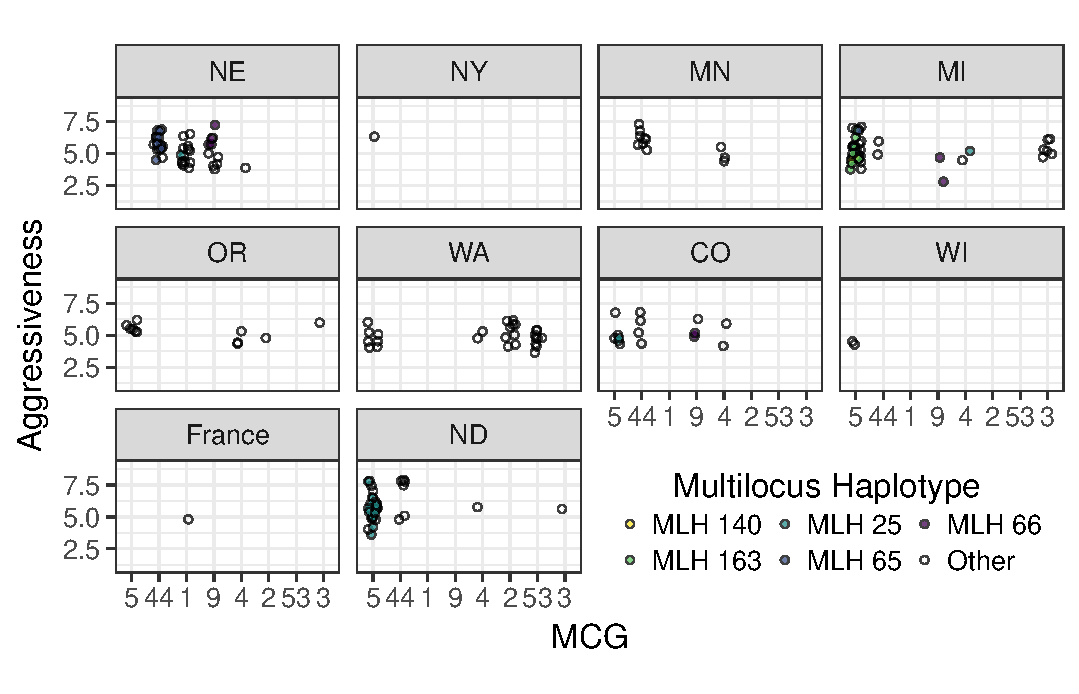
\includegraphics[width=1.00000\textwidth]{../../results/figures/publication/RMM-aggressiveness.pdf}
\caption{Strip plot of aggressiveness for the eight most abundant MCGs
partitioned by region. Filled circles indicate one of the five most
abundant MLHs and open circles indicate a MLH of lesser
abundance.}\label{mcg-mlh-region-aggressiveness}
\end{figure}

\begin{figure}
\centering
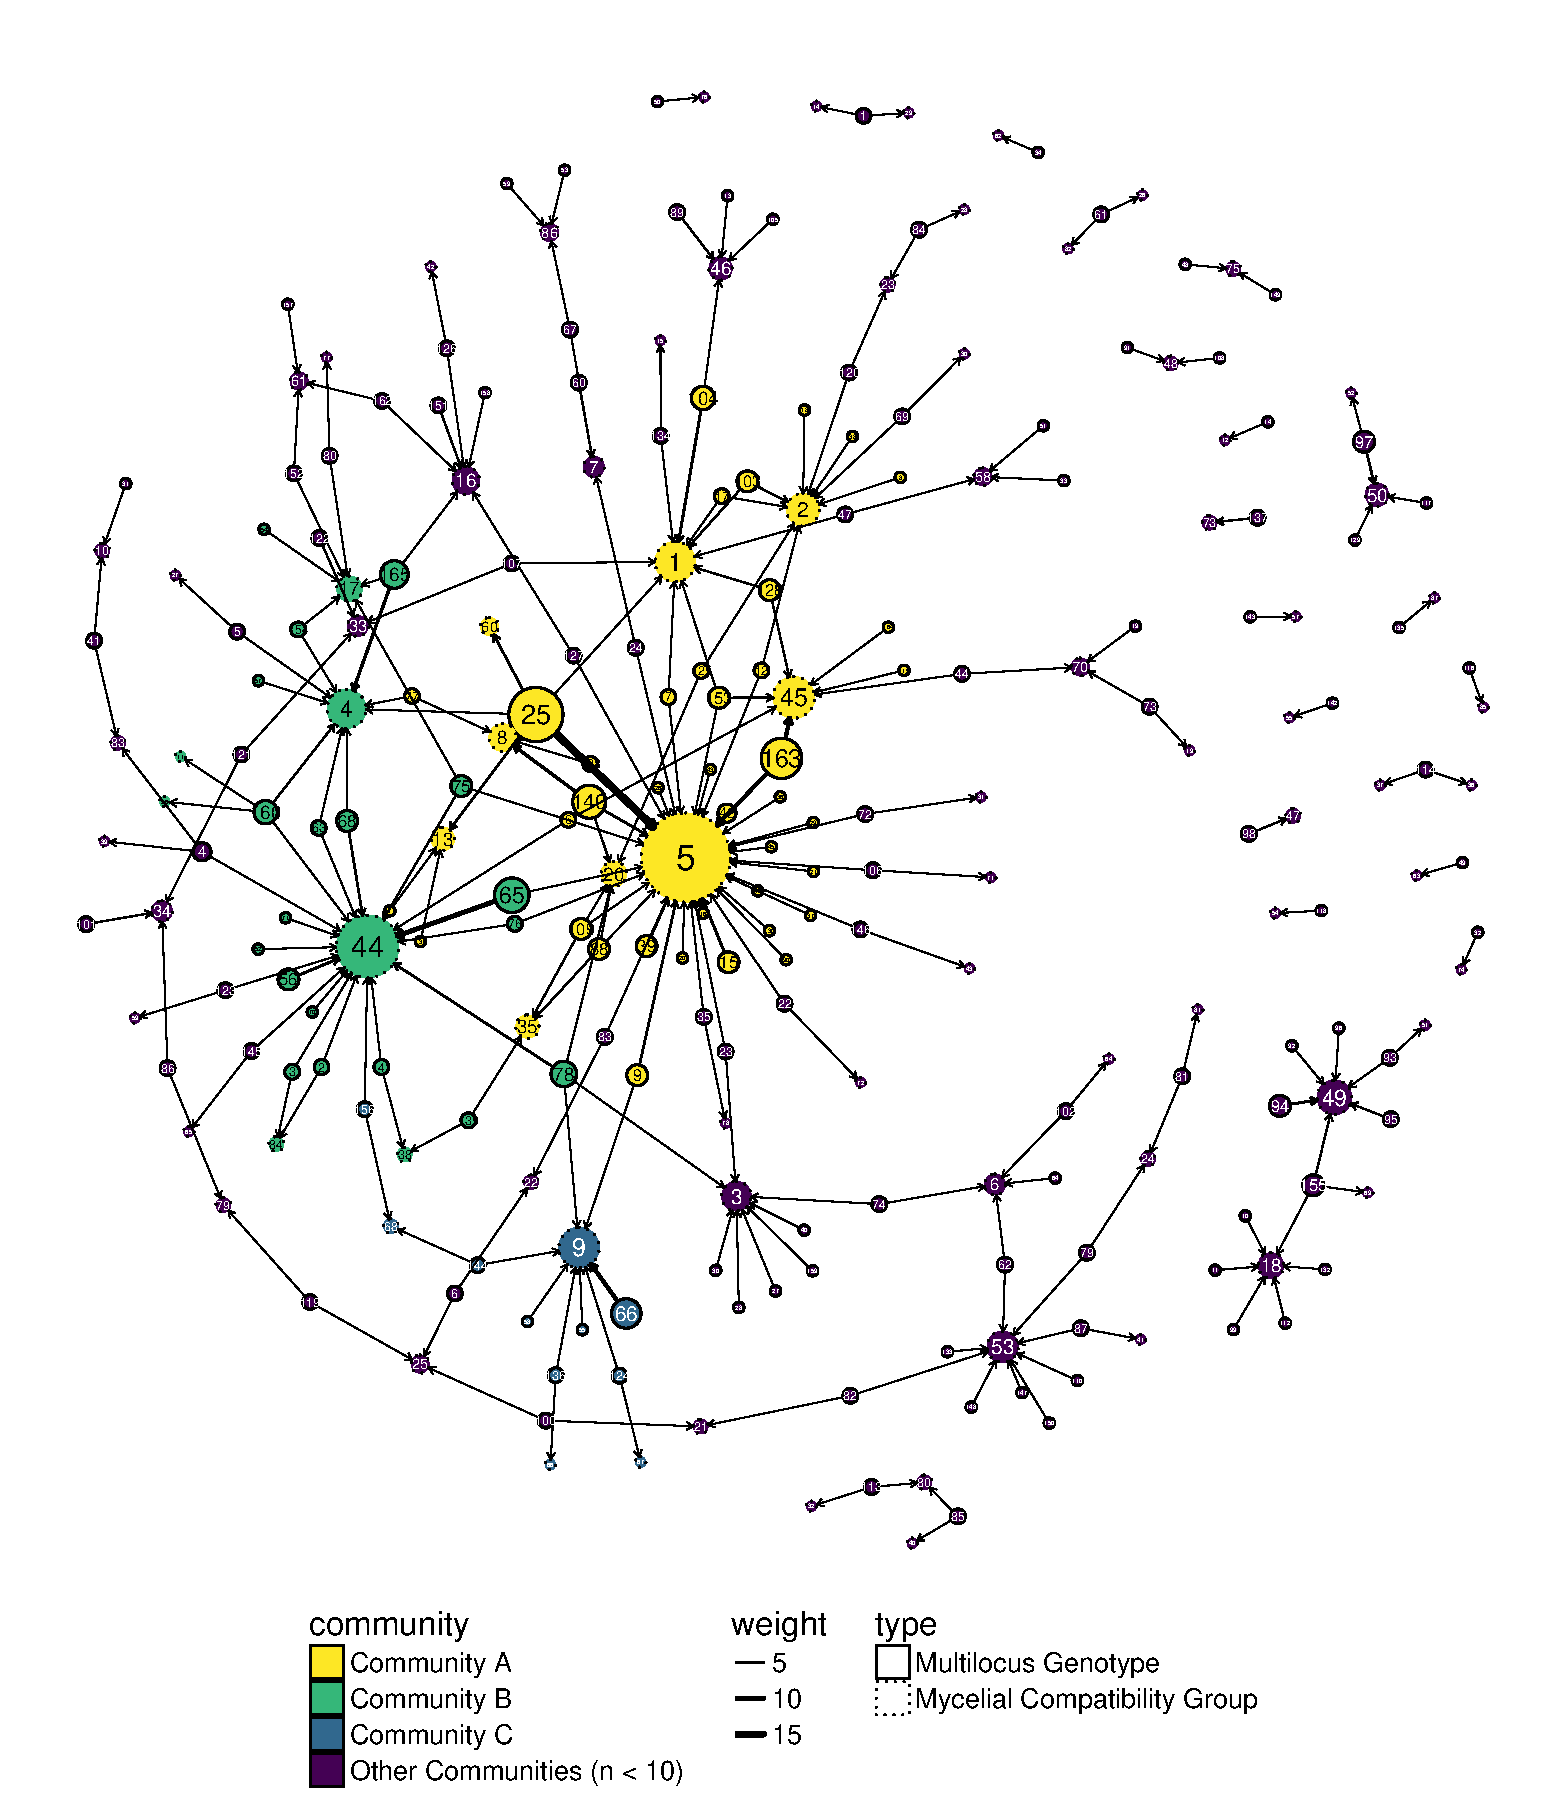
\includegraphics[width=1.00000\textwidth]{../../results/figures/publication/full-graph.pdf}
\caption{Graph showing complex associations between Mycelial
Compatibility Groups (MCG) (dotted nodes) and Multilocus Haplotypes
(MLH) (full nodes) where the number in each node represents the MLH/MCG
assignment. Node size reflect the number of samples represented by each
node (circle). Edges (arrows) point from MLH to MCG where the weight
(thickness) of the edge represents the number of samples shared. Node
color represents the community assignment based on the walktrap
algorithm with a maximum of four steps (Pons \& Latapy, 2006). An
interactive version of this network can be recreated using the code in
the ``Interactive visualizations'' section of the mlg-mcg.md file in the
supplementary information (Direct Link:
\url{https://github.com/everhartlab/sclerotinia-366/blob/master/results/mlg-mcg.md\#interactive-visualizations})
(Kamvar et al., 2017).}\label{fullgraph}
\end{figure}

\begin{figure}
\centering
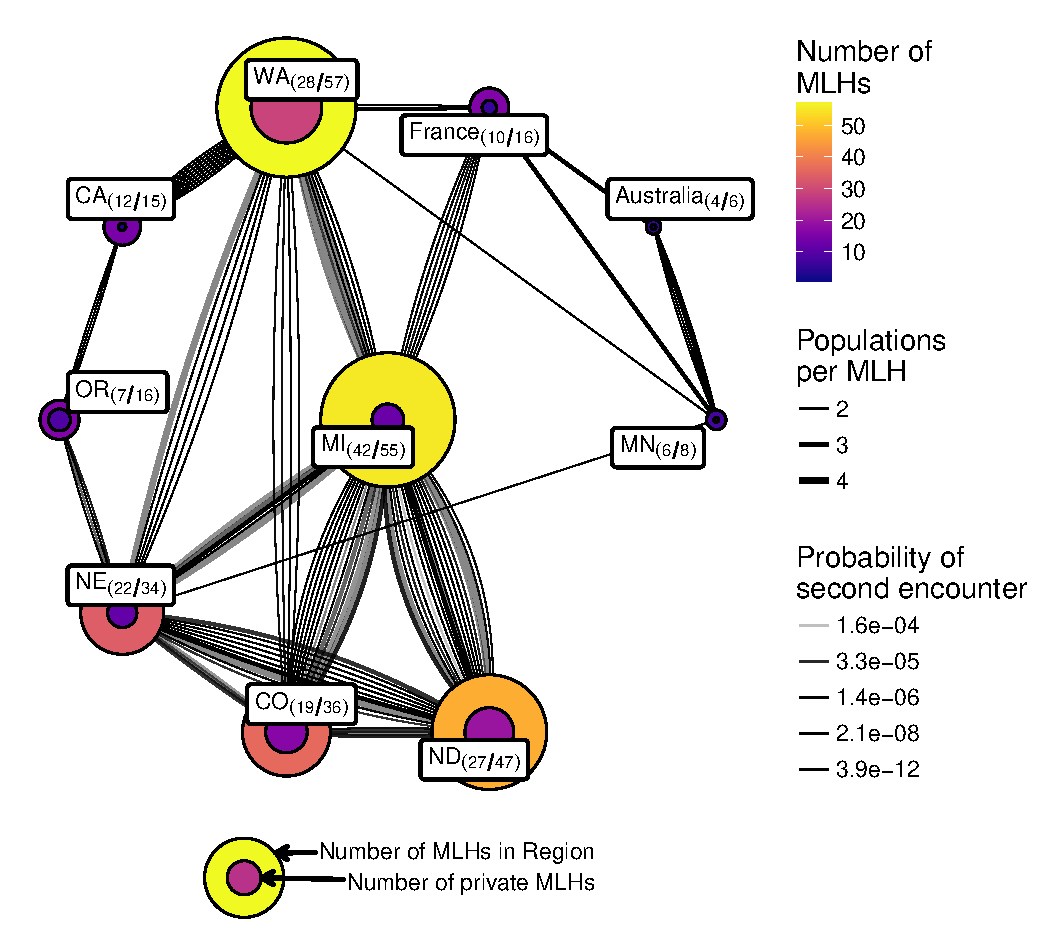
\includegraphics[width=1.00000\textwidth]{../../results/figures/publication/mlg-16.pdf}
\caption{Network of populations (nodes/circles) and their shared
multilocus haplotypes (MLH) (edges/lines) haplotyped over 16 loci. Each
node is labeled with \textbf{name (number of MLHs shared/number of MLHs
total).} The shade and area of the nodes are proportional to the number
of unique MLHs within the node and the inner nodes are proportional to
the number of private MLHs to the region (bottom legend). Each edge
represents a single MLH where its thickness represents the number of
populations that share the MLH and the shade represents the value of
\(P_{sex}\), or the probability of encountering that MLH from two
independent meiotic events.}\label{community-graph16}
\end{figure}

\begin{figure}
\centering
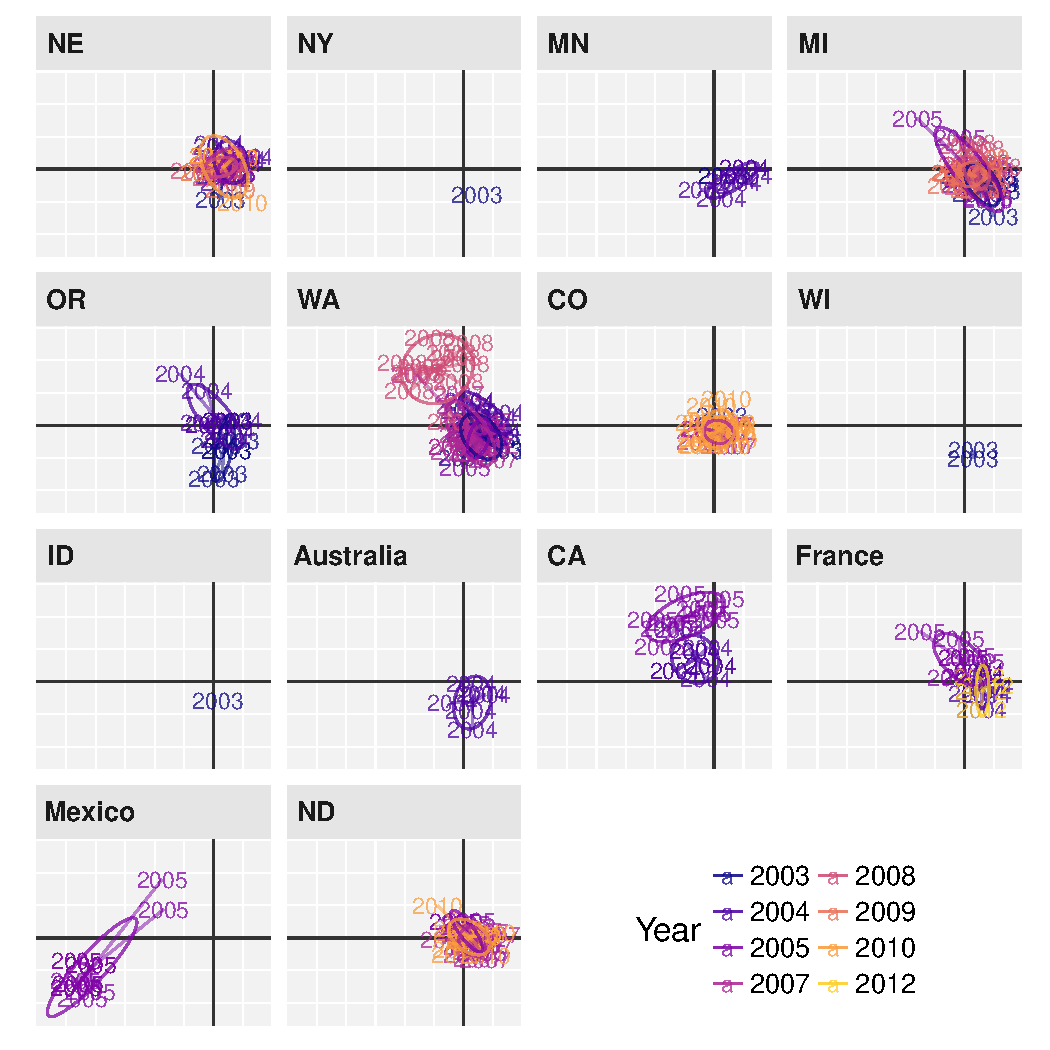
\includegraphics[width=1.00000\textwidth]{../../results/figures/publication/dapc_region_year.pdf}
\caption{Scatter plot of Discriminant Analysis of Principal Components
on Regions and Years showing temporal variation across all Regions.
Points (text labels) represent observed individuals connected to the
population centroids with ellipses representing a 66\% confidence
interval for a normal distribution. The center of each component is
represented as black grid lines.}\label{DAPC-RY-FULL}
\end{figure}

\newpage

